% ─────────────────────────────────────────────────────────────────────────────
% Sec. 3  Method. Every number here matches foveatile_internvl.py / foveatile_config.py (frozen v1.0).
% ─────────────────────────────────────────────────────────────────────────────
\section{Method}
\label{sec:method}

\method decides \emph{which} image regions to encode before any of them reaches the vision encoder.
Given a token budget, it keeps a low-resolution view of the whole image, uses the VLM itself to rank the
high-resolution tiles by their relevance to the question, and streams only the selected tiles into the
KV cache. Tiles that are not selected are never encoded. As a result, the vision encoder, the language
model, and the KV cache operate on a number of tokens set by the budget, not by the input
resolution. \cref{fig:method} gives an overview; \cref{alg:foveatile} lists the entire procedure.

\begin{figure*}[t]
  \centering
  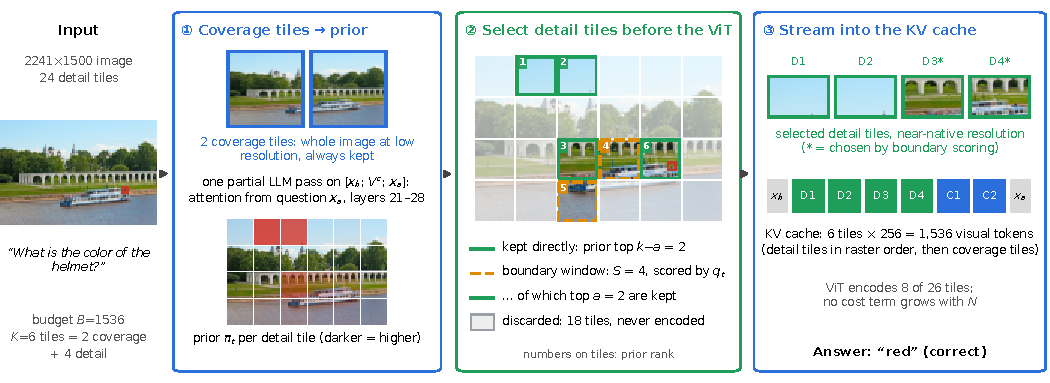
\includegraphics[width=\linewidth]{figures/fig_overview.pdf}
  \caption{\textbf{Overview of \method.} The image is represented at two scales: $m$ coverage tiles
  that show the whole image at low resolution, and a grid of $N$ detail tiles at near-native resolution.
  A single partial forward pass over the coverage tiles yields a question-aware prior over the detail
  tiles. The top-ranked tiles are kept directly, the tiles at the selection boundary are re-scored with
  question attention, and all other tiles are discarded \emph{before} the vision encoder. The selected
  tiles are streamed into the KV cache, so compute and memory are bounded by the budget $K$ rather than
  by $N$. Example from V$^*$~Bench~\cite{vstar} with $B=1536$ ($K=6$); the 3:2 image fits a $2\times1$ coverage grid, so the
  spare slot goes to the detail tiles. The prior ranks the target tile only sixth, and boundary scoring
  recovers it.}
  \label{fig:method}
\end{figure*}

% ─────────────────────────────────────────────────────────────────────────────
\subsection{Preliminaries: where the cost of high resolution comes from}
\label{sec:prelim}

We build on dynamic-resolution VLMs~\cite{internvl15}, using InternVL3.5~\cite{internvl35} as the running
example.
An image of size $W\times H$ is resized to a grid of $c\times r$ tiles of $448\times448$ pixels, where
$(c, r)$ is the grid whose aspect ratio is closest to $W/H$ subject to $N=cr\le N_{\max}$; a global
thumbnail is appended when $N>1$. Each tile is encoded independently by the vision encoder, and
pixel shuffle followed by an MLP projector turns it into $n=256$ visual tokens. The language model
then prefills the sequence
\begin{equation}
  [\,\mathbf{x}_b;\ \mathbf{V}_1;\ \dots;\ \mathbf{V}_{N+1};\ \mathbf{x}_a\,],
  \label{eq:seq}
\end{equation}
where $\mathbf{x}_b$ is the text before the image (system prompt and user prefix), $\mathbf{V}_t\in
\mathbb{R}^{n\times d}$ are the tokens of tile $t$, and $\mathbf{x}_a$ is the question, the answer
instruction, and the assistant prefix.

Every stage of this pipeline grows with $N$: vision-encoder compute is $\mathcal{O}(N)$, the prefill
of the language model is $\mathcal{O}(N)$ in its linear layers and $\mathcal{O}(N^2)$ in attention, and
the KV cache is $\mathcal{O}(N)$. With the cap $N_{\max}=47$ used in our experiments, a 4K image already
yields 24 to 45 tiles (6K to 12K visual tokens); without a cap, an 8K image yields 188 tiles (48K
visual tokens).
Token-pruning methods remove tokens \emph{after} they are computed. VisionZip~\cite{visionzip} prunes
after the vision encoder, so the encoder still sees all $N$ tiles. FastV~\cite{fastv},
SparseVLM~\cite{sparsevlm}, and IF-Prune~\cite{ifprune} prune inside the language model, so the
encoder and the first layers still process all $nN$ tokens, and the peak memory of prefill is still
set by $N$.

\paragraph{Problem setting.}
Given a budget of $B$ visual tokens, \ie $K=\lfloor B/n\rfloor$ tiles, we want to choose \emph{before
encoding} which tiles to keep, such that the vision encoder, the language model, and the KV cache
each process $\mathcal{O}(K)$ tokens independently of $N$. The method is training-free and uses no
model other than the VLM itself.

% ─────────────────────────────────────────────────────────────────────────────
\subsection{Coverage tiles and detail tiles}
\label{sec:scales}

\method represents the image at two scales and splits the $K$ tile slots between them.

\paragraph{Coverage tiles.} The whole image is resized to a $c_c\times r_c$ grid of at most $m$ tiles,
where $m=\max(1,\lfloor K/2\rfloor)$. The official tiling optimizes only the aspect-ratio match and
often leaves part of such a budget unused. We instead pick the grid with the \emph{most} tiles,
$c_c r_c\le m$, among those whose aspect-ratio distortion is at most $1.75\times$, so that the coverage
tiles use their share of the budget. The coverage tiles are always kept. They give the model the global layout
and context of the image, and they are the input to the prior (\cref{sec:prior}). HiRED~\cite{hired} and
GlobalCom2~\cite{globalcom2} also use a global view to decide how many tokens each crop keeps, but they
rank crops by vision-encoder attention without the question, and they still encode every crop.

\paragraph{Detail tiles.} The detail tiles are the official $c\times r$ grid with $N\le N_{\max}=47$
tiles, \ie close to native resolution. \method keeps $k=K-c_cr_c$ of them, so slots that the coverage grid
cannot fill go to detail tiles.

With $m=1$ the coverage tile reduces to the official thumbnail. Splitting the budget evenly between
the two scales is a calibrated choice (\cref{sec:impl}): document-style questions benefit from more
coverage, while questions about small, local details need detail tiles.

% ─────────────────────────────────────────────────────────────────────────────
\subsection{Question-aware prior from coverage tiles}
\label{sec:prior}

To rank the detail tiles without encoding them, we ask the VLM where it looks when it reads the question
against the low-resolution view. This builds on the observation that MLLMs attend to the relevant region
even when they cannot resolve its details~\cite{vicrop}. Zoom-in methods exploit this by searching over
crops with repeated forward passes or an external retriever~\cite{vstar,zoomeye,dyfo,rap}; we instead
compute a single prior from the coverage tiles, before any detail tile is encoded. We run the language
model on
$[\,\mathbf{x}_b;\ \mathbf{V}^{c};\ \mathbf{x}_a\,]$, where $\mathbf{V}^{c}\in\mathbb{R}^{nm\times d}$
are the coverage tokens, and stop after layer $l_{\text{hi}}$. Let $\mathbf{A}^{(l)}$ be the
head-averaged attention of layer $l$. The saliency of coverage patch $j$ is the attention it receives
from all text positions after the image, averaged over a band of middle-to-late layers
$\mathcal{L}_p=\{l_{\text{lo}},\dots,l_{\text{hi}}\}$, where visual information is transferred to the
question tokens~\cite{crossmodalflow}:
\begin{equation}
  s_j=\frac{1}{|\mathcal{L}_p|}\sum_{l\in\mathcal{L}_p}\frac{1}{|\mathbf{x}_a|}
      \sum_{i\in\mathbf{x}_a}\mathbf{A}^{(l)}_{i,j}.
  \label{eq:saliency}
\end{equation}
After min-max normalization, each coverage patch is assigned to the detail tile that contains its
center in normalized image coordinates, and the prior of detail tile $t$ is the mean saliency of its
patches, $\pi_t=\frac{1}{|P_t|}\sum_{j\in P_t}s_j$, again min-max normalized.

This pass costs a single forward over $|\mathbf{x}_b|+nm+|\mathbf{x}_a|$ tokens through
$l_{\text{hi}}$ of the $L$ layers, which is independent of $N$. We compute only the attention rows of
$\mathbf{x}_a$ in \cref{eq:saliency} and keep the fused attention kernel for the forward pass, so the
full attention matrix is never materialized. The pass also produces the KV cache of the prefix
$[\,\mathbf{x}_b;\ \mathbf{V}^{c}\,]$, which the next stage reuses.

% ─────────────────────────────────────────────────────────────────────────────
\subsection{Boundary scoring with question attention}
\label{sec:boundary}

The prior is computed at low resolution, so it is reliable for clearly relevant regions but uncertain
near the cut-off. \method therefore spends additional computation only on the tiles at the selection
boundary (\cref{fig:boundary}), similar to retrieve-then-rerank pipelines that apply an expensive scorer
only to the candidates of a cheap first stage~\cite{monobert}. Let the detail tiles be sorted by $\pi_t$, let $k$ be the number of
detail slots, and let $S$ be the size of the scoring window. With $a=\min(k,\lfloor S/2\rfloor)$:
\begin{enumerate}
  \item the top $k-a$ tiles are \emph{kept directly} (encoded, not scored);
  \item the next $S$ tiles form the \emph{boundary window}; they are encoded and scored, and the $a$
        highest-scoring ones are kept;
  \item all remaining tiles are \emph{discarded} and never reach the vision encoder.
\end{enumerate}
The score of a boundary tile $t$ is its question attention at layer $l_q$, measured in the context of
the coverage tiles:
\begin{equation}
  q_t=\frac{1}{|\mathbf{x}_a|}\sum_{i\in\mathbf{x}_a}\ \sum_{j\in\mathbf{V}_t}
      \mathbf{A}^{(l_q)}_{i,j}
  \quad\text{on}\quad [\,\mathbf{x}_b;\ \mathbf{V}^{c};\ \mathbf{V}_t;\ \mathbf{x}_a\,].
  \label{eq:qattn}
\end{equation}
Because the prefix $[\,\mathbf{x}_b;\ \mathbf{V}^{c}\,]$ is shared by all candidates, its keys and values
for layers $1,\dots,l_q$ are taken from the prior pass, as in prompt caching~\cite{promptcache}. Each candidate therefore costs one pass of
$n+|\mathbf{x}_a|$ tokens through $l_q$ layers, and this is mathematically identical to a full forward
over the sequence in \cref{eq:qattn}. Since $q_t$ depends only on tile $t$ and the question, the top-$a$
selection can be made on the fly with a size-$a$ min-heap while the window is streamed, without holding
all candidates in memory. Setting $S=0$ reduces \method to prior-only selection.

\begin{figure}[t]
  \centering
  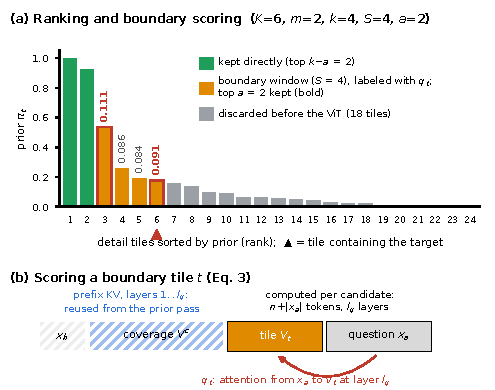
\includegraphics[width=\linewidth]{figures/fig_boundary.pdf}
  \caption{\textbf{Boundary scoring} on the example of \cref{fig:method}. (a) Detail tiles sorted by the
  prior $\pi_t$. The top $k-a$ tiles are kept directly, the next $S$ tiles are scored by question
  attention $q_t$ (\cref{eq:qattn}) and the top $a$ are kept, and the rest are discarded before the
  vision encoder. The target tile is ranked sixth by the prior but has the second-highest $q_t$ in the
  window. (b) Each candidate reuses the prefix KV cache of $[\mathbf{x}_b;\mathbf{V}^c]$ from the prior
  pass, so only $n+|\mathbf{x}_a|$ tokens are processed per tile.}
  \label{fig:boundary}
\end{figure}

% ─────────────────────────────────────────────────────────────────────────────
\subsection{Streaming KV construction}
\label{sec:streaming}

\method builds the KV cache incrementally. It first prefills $\mathbf{x}_b$, then encodes the coverage
tiles and runs the prior. The candidate detail tiles, \ie the directly kept tiles and the boundary window,
are encoded in raster order in micro-batches of four tiles; boundary tiles are scored as they arrive and
enter or leave the size-$a$ pool. Once selection is final, the selected detail tiles are written to the
KV cache in raster order, followed by the $m$ coverage tiles. This mirrors the order seen in training,
where grid tiles precede the global thumbnail. The visual tokens are prefilled in chunks of 1{,}024
tokens with contiguous position ids after $\mathbf{x}_b$. Finally, $\mathbf{x}_a$ is prefilled and the
answer is decoded from the resulting cache of at most $|\mathbf{x}_b|+nK+|\mathbf{x}_a|$ tokens. The
visual tokens resident in memory never exceed about $k+m$ tiles plus one micro-batch, \ie
$\mathcal{O}(K)$.

\begin{algorithm}[t]
\caption{\method inference for one image--question pair}
\label{alg:foveatile}
\begin{algorithmic}[1]
\Require image $I$, text $\mathbf{x}_b,\mathbf{x}_a$, budget $K$ tiles, window $S$
\State $m\gets\max(1,\lfloor K/2\rfloor)$;\ \ $a\gets\min(k,\lfloor S/2\rfloor)$ with $k=K-c_cr_c$
\State $\mathcal{C}\gets$ KV cache after prefilling $\mathbf{x}_b$
\State $\mathbf{V}^{c}\gets\textsc{Encode}(\textsc{CoverageTiles}(I,m))$
\State $\pi,\ \mathcal{C}_{\text{pre}}\gets\textsc{Prior}(\mathbf{x}_b,\mathbf{V}^{c},\mathbf{x}_a)$
  \Comment{\cref{eq:saliency}, layers $\le l_{\text{hi}}$}
\State $\sigma\gets$ detail tiles of $I$ sorted by $\pi$ (descending)
\State $D\gets\sigma[1{:}k-a]$;\ \ $W\gets\sigma[k-a+1{:}k-a+S]$ \Comment{rest: never encoded}
\State $\mathcal{H}\gets$ empty min-heap of capacity $a$
\For{each micro-batch $T\subset D\cup W$ in raster order}
  \State $\{\mathbf{V}_t\}_{t\in T}\gets\textsc{Encode}(T)$
  \For{$t\in T\cap W$}
    \State push $(q_t,\mathbf{V}_t)$ into $\mathcal{H}$ \Comment{\cref{eq:qattn}, reuses $\mathcal{C}_{\text{pre}}$}
    \If{$|\mathcal{H}|>a$} pop the lowest-scoring tile from $\mathcal{H}$ \EndIf
  \EndFor
\EndFor
\State $\mathcal{C}\gets\textsc{Prefill}(\mathcal{C},\ \text{tiles }D\cup\mathcal{H}\text{ in raster order},\ \mathbf{V}^{c})$
\State $\mathcal{C}\gets\textsc{Prefill}(\mathcal{C},\mathbf{x}_a)$;\ \ \Return $\textsc{Decode}(\mathcal{C})$
\end{algorithmic}
\end{algorithm}

\paragraph{Cost.}
\cref{tab:complexity} summarizes the cost per image. \method encodes $c_cr_c+(k-a)+S=K-a+S$ tiles. Its
language-model work consists of the prior pass over $|\mathbf{x}_b|+nm+|\mathbf{x}_a|$ tokens
($l_{\text{hi}}$ layers), $S$ scoring passes of $n+|\mathbf{x}_a|$ tokens ($l_q$ layers), and the main
prefill of $nK$ visual tokens. Every term depends on the budget $K$ and the window $S$, but none depends
on the number of tiles $N$. The KV cache is bounded by the budget. In contrast, every method that prunes
after encoding pays $\mathcal{O}(N)$ vision compute, and methods that prune inside the language model
also pay $\mathcal{O}(N)$ in the layers before pruning.

\begin{table}[t]
  \centering
  \small
  \setlength{\tabcolsep}{4pt}
  \begin{tabular}{lccc}
    \toprule
    Method & ViT & LLM prefill & KV cache \\
    \midrule
    Uncompressed & $N$ & $N$ & $N$ \\
    VisionZip & $N$ & $K$ & $K$ \\
    FastV, SparseVLM & $N$ & $N\!\to\!K$ & $\approx K$ \\
    IF-Prune & $N^{\ddagger}$ & $N\!\to\!K$ & $\approx K$ \\
    \method (ours) & $K{-}a{+}S$ & $K{+}m{+}S^{\dagger}$ & $K$ \\
    \bottomrule
  \end{tabular}
  \caption{\textbf{Cost per image} of VisionZip~\cite{visionzip}, FastV~\cite{fastv},
  SparseVLM~\cite{sparsevlm}, IF-Prune~\cite{ifprune}, and \method, in units of tiles ($n=256$ tokens
  each), with $N$ detail tiles and a budget of $K$ tiles; text tokens are omitted. $N\!\to\!K$: all $N$ tiles pass through the layers
  before pruning, $K$ remain after. $^{\ddagger}$IF-Prune also runs a 1B guide VLM on all $N$ tiles.
  $^{\dagger}$The $m$ coverage tiles pass through the first $l_{\text{hi}}$ layers for the prior, and each of the
  $S$ boundary tiles through the first $l_q$ layers for scoring. Only \method is independent of $N$.}
  \label{tab:complexity}
\end{table}

% ─────────────────────────────────────────────────────────────────────────────
\subsection{Hyperparameters and calibration}
\label{sec:impl}

\method has no trained parameters. The coverage fraction $m/K$, the window $S$ as a function of the
budget, and the default budget are set once on held-out data and frozen for all test sets. The
calibration sets are 600 questions sampled from the InfoVQA \emph{train}
split and 600 questions from MME-RealWorld excluding its Lite subset and images, so they share no
questions or images with any test set. On these sets, $m/K=0.5$ is within 0.1 points of the best
average accuracy and has the most stable worst-task accuracy. With $m=1$, \ie the thumbnail alone as coverage, accuracy is
about 5 points lower on average. Disabling boundary scoring ($S=0$) costs up to 10.8 points on remote
sensing questions, while windows up to four times larger than ours give no reliable gain. We therefore
use $S=\{5,4,4,3,3\}$ for $B=\{1024,1536,2048,2560,3072\}$. The default budget is $B=1536$ ($K=6$,
$m=3$, $S=4$), where held-out accuracy saturates. The attention layers were fixed in preliminary
experiments before this protocol: for InternVL3.5-8B ($L=36$) we use $\mathcal{L}_p=\{21,\dots,28\}$
and $l_q=20$. The full protocol, including deviations from our pre-registered rules, is given in the
supplementary material.

% NOTE: L_p and l_q were chosen on InfoVQA val before the held-out protocol existed
% (docs/04_calibration_protocol.md, 1.8.3 note). Disclose this in the supplementary.
